%\documentclass[12pt,letter]{report}
\documentclass[11pt,oneside,openany,letter]{book}
\usepackage[colorlinks=true,bookmarksnumbered,linktocpage,pdftex]{hyperref}
\usepackage{hyperref}
\usepackage[activeacute,spanish]{babel}
\usepackage[utf8]{inputenc}
\usepackage{amsmath}
\usepackage{float}
\usepackage{epsfig}
\usepackage{graphicx}
\usepackage{titlesec}
\usepackage{multirow}
\usepackage{graphicx}
\usepackage{caption}
\usepackage{subcaption}
\usepackage{color}
\usepackage{calc}
\usepackage[nottoc]{tocbibind}
\usepackage{titletoc}
\usepackage{capt-of}
\usepackage{verbatim}
\usepackage{setspace}
\spacing{1.5}
\usepackage[titletoc,title]{appendix}
\usepackage[left=3cm, right=3cm,top=3cm, bottom=2.5cm]{geometry}
\usepackage[table,xcdraw]{xcolor}

\newcommand{\bigrule}{\titlerule[1mm]}
\definecolor{c1}{rgb}{0,0.5,0}
\definecolor{c2}{rgb}{0.9,.0,0}
\definecolor{c3}{rgb}{.465,.535,.605}%color del panel
\definecolor{c4}{rgb}{.6,.6,.6}%color de los botones del panel

\hypersetup{linkcolor=blue}                         
\hypersetup{citecolor=red}

%%%%FORMA DE LOS CAPITULOS SECCIONES...ETC%%%%%%

%========================================
% Formato de capítulos y secciones
%\newcommand{\esp}{\rule{0in}{3ex}} %para crear espacios en las tablas
\usepackage{titlesec}
\titleformat{\section}[hang]{\bfseries} {\Large\thesection}{10pt}{\Large}[{\titlerule[0pt]}]
 % Para hacer una línea debajo de cada sección
\titleformat{\chapter}[display] % cambiamos el formato de los capítulos
{\bfseries\Huge} % por defecto se usarán caracteres de tamaño \Huge en negrita
{ \filleft % texto alineado a la derecha
 \Large\chaptertitlename\ % "Capítulo" o "Apéndice" en tamaño \Large en lugar de \Huge
 \Large\thechapter} % número de capítulo en tamaño \Large
{0mm} % espacio mínimo entre etiqueta y cuerpo
{\filleft} % texto del cuerpo alineado a la derecha
[\vspace{0.5mm} \bigrule] % después del cuerpo, dejar espacio vertical y trazar línea horizontal gruesa



\setlength{\parskip}{10pt} %espacio entre párrafos
\makeatletter
\newcommand\figcaption{\def\@captype{figure}\caption}
\makeatother


%%%%%%%%%% NEW COMANDS %%%%%%%%%%%%%%%%%%%%%%%%%%%%%%%%%%%%%%%%%55

%%%%%%%%%%%%%%%%%%%%%%%%%%%%%%%%%%%%%%%%%%%%%%%%%%%%%%%%%%%%%%%%%%%%%%%%%%%%%%
\parindent0cm %Sangria
\parskip0.5cm %Espacio entre prrafos.
\baselineskip0cm
\begin{document}
\begin{titlepage}


\centering {\Large {\sc  ELVES: Fenómenos Luminosos Transitorios de la alta Atmósfera}}

\vfill

\centering {\Large \textbf{Adriana Carolina Vásquez Ramírez} $^{1}$}

\vfill

\centering {\Large \textbf{Director:} Luis A. Núñez $^{1}$}

\centering {\Large \textbf{Co-Director:} Enrico Arnone $^{2}$}

\centering {\Large \textbf{Co-Director:} Roberto Mussa $^{3}$}

\vfill

$^{1}$  Escuela de F\'isica, Universidad Industrial de Santander \\
$^{2}$ Departamento de F\'isica, Universidad de Tur\'in
\\
$^{3}$ Instituto Nacional de F\'isica Nuclear,  Secci\'on de Tur\'in\\
\vfill

\centering {\Large Universidad Industrial de Santander\\Facultad de
Ciencias\\Escuela de F\'{i}sica\\2020}
\end{titlepage}

\tableofcontents
\listoffigures
%\listoftables
%\newpage

%\chapter*{Resumen}
%que son los tles
%que son los elves
%relaci'on entre tles, rayos y gammas

%%%%%%%%%%%%%%%%%%%%%%
%%%%% CHAPTER 1  %%%%%
%%%%%%%%%%%%%%%%%%%%%%
\chapter*{Introducci\'on}\label{introduccion}
\addcontentsline{toc}{chapter}{Introducci\'on}
\begin{figure}
    \centering
    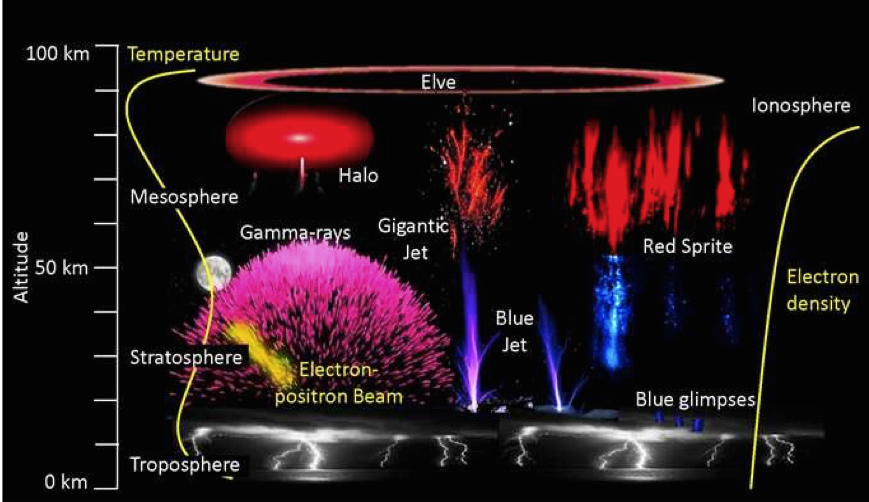
\includegraphics[scale=0.7]{figures/tle_and_tgf.png}
    \caption[Fenómenos de la atmósfera superior generados por tormentas eléctricas]{Fenómenos de la atmósfera superior generados por tormentas eléctricas, incluyendo Destellos de Rayos Gamma Terrestres (TGF) y Emisiones Luminosas Transitorias (TLE). En esta figura se observan las dimensiones y las altitudes típicas en las que ocurren estos fenómenos. Las descargas eléctricas incluyen ``destellos azules'' en la parte superior de las tormentas eléctricas, \textit{Blue Jets} , \textit{Jets} Gigantes, \textit{Sprites}, Halos, y ELVES (Tomado de \cite{Gaskill2018}).}
    \label{fig:tle_and_tgf}
\end{figure}
Desde el siglo pasado se empezaron a reportar fen\'omenos luminosos ascendentes que se produc\'ian por encima de las tormentas el\'ectricas, por lo que se denominaban rayos de nube a la alta atmósfera, nube al espacio o nube a la ionosfera. M\'as adelante, Winckler \cite{FranzEtal1990} captur\'o con una c\'amara de v\'ideo de alta sensibilidad, las primeras imágenes de lo que hoy se conoce como un \textit{Sprite}. El v\'ideo revel\'o un rayo ascendente de columnas gemelas de luz, con longitudes de decenas de kil\'ometros, lo que llam\'o la atenci\'on del programa de vuelos espaciales de Estados Unidos, que ya hab\'ia tenido encuentros desafortunados con estos rayos \cite{UmanRakov2003}. Fue as\'i como surgieron varios programas para el estudio de los Eventos Luminosos Transitorios, denotados como TLE. 

Los TLE son emisiones cortas de luz que ocurren encima de las tormentas eléctricas, en las capas más altas de la atmósfera, es decir, en la estratosfera, la mesosfera y en la parte baja de la ionosfera. Estos eventos se originan a partir de las descargas eléctricas entre las nubes, o entre las nubes y el suelo \cite{DwyerUman2014}. Hasta ahora, se han reportado los siguientes tipos de TLE: \textit{Sprites}, \textit{Blue Starters} o \textit{glimpses}, \textit{Blue Jets}, \textit{Jets} Gigantes, ELVES y Halos. La dinámica de estos fenómenos electromagnéticos, que involucra corrientes eléctricas, ondas electromagnéticas y gases ionizados, aún no se entiende por completo \cite{DwyerUman2014}. As\'i mismo, se han observado Destellos de Rayos Gamma Terrestres (TGF) provenientes de las tormentas eléctricas y las condiciones en las que se generan sigue siendo una pregunta abierta \cite{neubertEtal2020}. En la figura \ref{fig:tle_and_tgf} se muestran los diferentes fenómenos de la atmósfera superior producidos por tormentas eléctricas, incluyendo los TGF y los TLE. En ésta se puede observar la altitud característica de cada evento, así como el tamaño referencial de unos respecto a otros. 

Los ELVES son emisiones de luz difusa en forma de disco, que se produce cuando el pulso electromagn\'etico de una descarga el\'ectrica intersecta la ionosfera. Estos fen\'omenos ocurren con m\'as frecuencia que los dem\'as TLE \cite{chen2008}. Adem\'as, a diferencia de los \textit{Sprites} y los \textit{Blue Jets}, los ELVES son imperceptibles al ojo humano debido a su bajo brillo y corta duraci\'on ($\sim 1$ ms) \cite{FullekrugEtal2006}. Por lo general se detectan con c\'amaras de alta velocidad, arreglos de fot\'ometros o fotomultiplicadores, con resoluciones temporales del orden de los $\mu$s \cite{MussaCiaccio2012}. Existen varios programas como el ISUAL \cite{chen2008}, TARANIS \cite{lefeuvre2008taranis}, Firefly \cite{rowland2011nsf} y el ASIM \cite{neubertEtal2019}, diseñados para la observación de los ELVES desde la atm\'osfera. Por otro parte, el Observatorio Pierre Auger, diseñado para el estudio de Rayos Cósmicos de ultra alta energía, en el 2005 detectó por accidente un ELVES \cite{MussaCiaccio2012}, por lo que comenz\'o a explotar las caracter\'isticas de su Detector de Fluorescencia para el estudio de estos fenómenos. 

El objetivo de esta monografía es resumir la evolución que ha tenido la detección y el estudio de los ELVES. Gracias a la mejoría de la sensibilidad de los detectores, se ha pasado de capturarlos como un brillo difuso en el cielo \cite{BoeckEtal1992, Lyons1994A}, hasta medir la expansión lateral rápida de su luminosidad \cite{InanEtal1997}. Asimismo, se han descubierto estructuras de múltiples picos en sus trazas fotométricas \cite{Newsome2010, Mussa2019, aab2020}, cuyo análisis puede contribuir a entender mejor los procesos de los rayos que los producen \cite{Marshall2014, Da2015}. Sin embargo, quedan temas en discusión sobre la fenomenología de los ELVES y su relación con otros fenómenos como los TGF \cite{Liu2017, neubertEtal2020}, por lo que es necesario seguir ampliando la base de datos y profundizar en el análisis de estos fenómenos. 

El origen de los TLE y los TGF dependen principalmente del tipo de rayo producido en una tormenta, por lo que en el cap\'itulo \ref{tormentas} se describe el modelo de la estructura ideal de carga de las tormentas, los tipos de descargas, la fenomenolog\'ia y el problema de iniciaci\'on de los rayos, as\'i como su monitoreo y distribuci\'on global. En el cap\'itulo \ref{fenomenos}, se resumen las características principales de los fenómenos en la alta atmósfera, basadas en las observaciones que se han realizado con sat\'elites y detectores desde la superficie. Finalmente, en el capítulo \ref{deteccion} se listan los principales monitores de ELVES, haciendo enf\'asis en el Observatorio Pierre Auger que podr\'ia ser el mejor instrumento para observar estos eventos desde la superficie.  

%%%%%%%%%%%%%%%%%%%%%%%%%%%%%%%%%%%%%%%%%%%%%%%
\chapter{Tormentas eléctricas}\label{tormentas}
Las tormentas eléctricas se producen en nubes densas de gran extensión vertical, conocidas como cumulonimbos, que se forman a partir del vapor de agua transportado por potentes corrientes de aire ascendente. Este fenómeno meteorológico se distingue por la presencia de rayos y truenos, que usualmente van acompañados de vientos y lluvias fuertes, o a veces de granizo o de nieve. 

Por encima de estas tormentas, a diferentes altitudes de la atmósfera, ocurren los denominados Eventos Luminosos Transitorios. Para explicar el origen de estos fenómenos es necesario conocer la dinámica de las tormentas, así como sus características y distribución global. En las secciones siguientes se describe la estructura de carga más simple de las tormentas eléctricas, la fenomenología, terminología y propagación de los rayos en la atmósfera, así como su distribución global y las redes de monitoreo de rayos alrededor del mundo.  

\section{Estructura de carga de las tormentas}
\begin{figure}
    \centering
    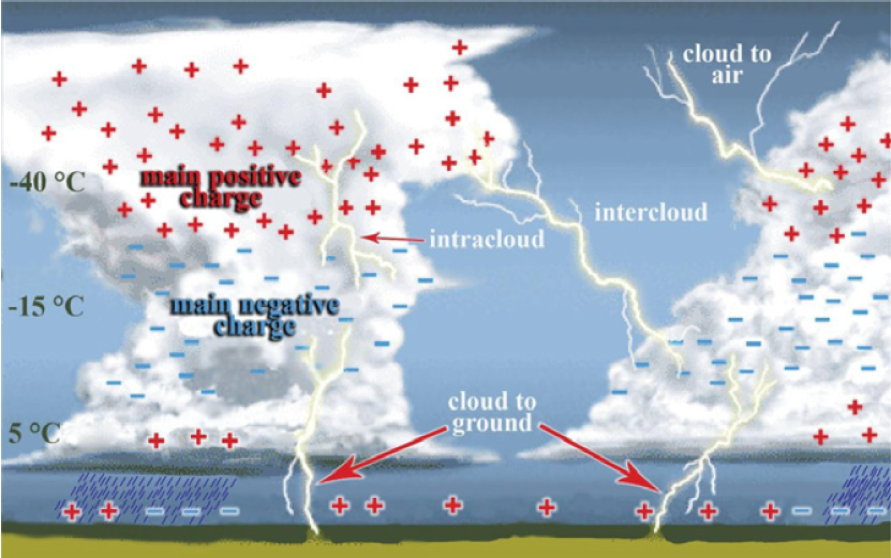
\includegraphics[scale=0.62]{figures/tormenta_modelo.png}
    \caption[Estructura de carga según el modelo de tripolo.]{Estructura de carga de dos tormentas simples aisladas. Según el modelo de tripolo la parte superior de la nube está dominada por la carga positiva principal, seguida de la capa negativa principal y una pequeña capa de carga positiva en la parte más baja. Además se muestran algunos sitios donde se pueden producir los rayos: dentro de la nube (IC), de nube a tierra (CG), entre dos nubes (CC) e incluso de nube al aire (CA). Tomado de \cite{DwyerUman2014}.}
    \label{fig:tormenta_modelo}
\end{figure}

La estructura de carga ideal de las tormentas eléctricas está definida por el modelo tripolar estándar, donde la nube tiene un centro de carga negativa principal, uno de carga positiva principal y un centro de carga positiva inferior (ver figura \ref{fig:tormenta_modelo}). Frecuentemente aparece una cuarta región de carga negativa significativa, llamada capa superior de apantallamiento, que expulsa las líneas de campo eléctrico producidas por las cargas de la tormenta eléctrica. Esta capa se forma debido a la mayor conductividad del aire limpio fuera de la nube, especialmente en la estratosfera sobre la tormenta \cite{DwyerUman2014}. 

El proceso de transferencia de la carga primaria en la nube, ocurre a través de las colisiones entre partículas de granizo blando y de pequeños cristales de hielo. El granizo es lo suficientemente pesado como para caer o permanecer inmóvil en las corrientes de aire ascendente de la tormenta, mientras que los cristales de hielo son lo suficientemente ligeros para dejarse llevar hacia arriba por esas corrientes \cite{DwyerUman2014}. 

Generalmente, el centro de carga negativa principal se encuentra concentrada en un rango de temperatura entre -10 $^{\circ}$C y -25 $^{\circ}$C independientemente de la altura del terreno debajo de la tormenta \cite{RakovEtal2003}, mientras que la región de carga positiva principal suele ser más difusa y reside en la zona superior de la nube. Dependiendo de la altura de la tormenta, la carga positiva superior puede oscilar entre los 8 km y 15 km de altitud \cite{DwyerUman2014}. La región positiva inferior se encuentra en el fondo de la nube visible; por ejemplo, en las tormentas de verano en Florida estaría por encima de los 2 km de altitud \cite{DwyerUman2014}. 





La estructura de carga en una tormenta eléctrica real puede ser más compleja que la que se muestra en la figura \ref{fig:tormenta_modelo}, es decir, puede variar en el tiempo debido a que los rayos depositan y reorganizan la carga dentro de la nube. Además, los campos eléctricos de las tormentas también varían dependiendo del tiempo, la ubicación y el tipo de tormenta, por lo que se debe tener cuidado al interpretar las observaciones a partir de un modelo específico \cite{DwyerUman2014}. Por otra parte, las dos nubes aisladas de la figura \ref{fig:tormenta_modelo} podrían ser parte de varias tormentas contiguas e interactivas que comprenden sistemas de tormentas más grandes y complejos. 



%%%%%%%%%%%%%%%%%%%%%%%%%%%
\section{Fenomenología de los rayos}\label{fenomenologia}
Los rayos se pueden definir como una chispa eléctrica muy larga que generalmente ronda entre 5 y 10 km de longitud, con algunos casos extremos de 100 km \cite{DwyerUman2014}. Las descargas eléctricas en las tormentas pueden durar alrededor de los 0.5 s \cite{DwyerUman2014} y producen pulsos electromagnéticos que se propagan en la atmósfera. Los rayos son los fenómenos más impresionantes y comunes en Geofísica, pues provocan la luz más brillante (relámpago) y el sonido más fuerte (trueno) en la Tierra, aunque su aparición aparentemente aleatoria en el espacio y el tiempo, la amplia gama de su variación temporal y el oscurecimiento de la nube que lo produce, hace que sean particularmente difíciles de estudiar.

\begin{figure}
    \centering
    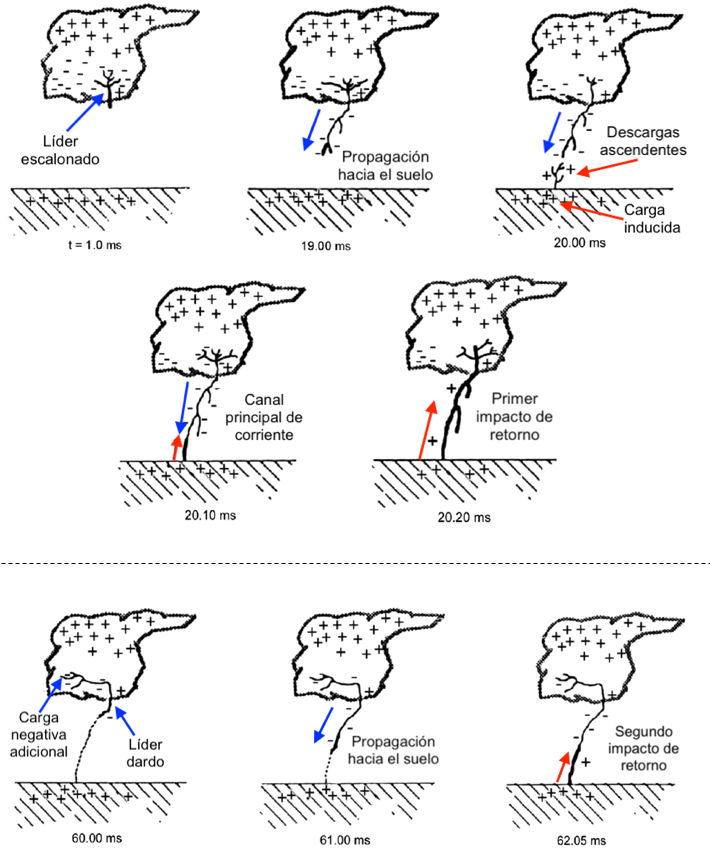
\includegraphics[scale=0.8]{figures/cg_development.png}
    \caption[Desarrollo de una descarga negativa de nube a tierra]{Esquema del desarrollo de una descarga negativa de nube a tierra. El l\'ider escalonado se va propagando hacia el suelo, induciendo una carga positiva sobre esta superficie. Una de estas descargas ascendentes entra en contacto con una rama del líder, determinando el canal principal de la corriente entre la nube y la superficie. A partir del primer impacto de retorno, la corriente se propaga continuamente hacia arriba con un tercio de la velocidad de la luz. Si existen cargas cercanas al canal principal, se genera un líder dardo que se propaga continuamente hacia el suelo, produciendo un segundo impacto de retorno en el canal principal. Figura modificada de \cite{DwyerUman2014}.}
    \label{fig:cg_development}
\end{figure}

Tomando en cuenta la estructura ideal de carga de las nubes (figura \ref{fig:tormenta_modelo}), se puede notar que no existe una sola ubicación para la iniciación de los rayos. Sin embargo, se han observado ciertos patrones que ayudan a clasificar las descargas eléctricas en dos categorías \cite{DwyerUman2014}: las que unen la brecha entre la carga de la nube y la tierra, y las que no. Las primeras se conocen como descargas de nube a tierra, denotadas como CG. Las segundas se dividen dependiendo del lugar donde se producen: dentro de la nube (denotada como IC), entre dos nubes (CC) y de la nube al aire (CA). Este grupo representa la mayoría de todas las descargas de rayos, siendo las IC las más comunes de todas las formas, seguidas de las CC y de las CA. 

Adem\'as, las descargas CG se clasifican en cuatro tipos, dependiendo del signo de la carga eléctrica y la dirección de propagación de rayo. La m\'as com\'un, denotada como -CG, es la que lleva carga negativa y se conecta con la carga positiva de la tierra. Un sistema típico de tormenta eléctrica pequeña produce un relámpago CG cada 20 s a 30 s durante 40 min a 60 min sobre una superficie típica de 100 km$^{2}$ a 300 km$^{2}$, mientras que los sistemas de tormentas grandes pueden producir más de un CG cada segundo, en áreas cien veces más grandes \cite{DwyerUman2014}.

El desarrollo de una descarga -CG, ilustrada en la figura \ref{fig:cg_development}, ocurre de la siguiente manera\cite{DwyerUman2014}: 

\begin{enumerate}
    \item Los electrones libres se mueven hacia la región de carga positiva en la parte más baja de la nube, neutralizando una fracción significativa de esta carga y continuando su viaje hacia el suelo en pasos escalonados de unos 10 m de longitud. A este mecanismo físico se le denomina líder escalonado y su propagaci\'on se observa en el intervalo $t=[\text{1.0},\, \text{19.00}]$ ms de la figura \ref{fig:cg_development}. 
    %Cada paso produce un pulso de luz visible, un pulso de energía de radiofrecuencia y un pulso de rayos X, en el rango de 200 keV. El tiempo entre los pasos luminosos es de $\sim 50\,\mu$s cuando el líder escalonado está muy por encima del suelo y de $\sim 10\,\mu$s cuando está cerca del suelo.
    
    \item En $t=$ 20.00 ms la carga negativa del l\'ider induce una carga positiva concentrada en el suelo y se inician descargas eléctricas ascendentes cargadas positivamente. 
    
    \item Una de estas descargas ascendentes entra en contacto con una rama del líder escalonado ($t=$ 20.10 ms), determinando el punto de impacto del rayo y el canal principal de la corriente entre la nube y el suelo.
    
    \item La corriente y la alta luminosidad del canal se generan en un proceso llamado el primer impacto de retorno, donde la carga positiva se propaga continuamente hacia arriba a una velocidad típicamente entre un tercio y la mitad de la velocidad de la luz ($t=$ 20.20 ms). El impacto de retorno calienta el aire, que se expande y produce los truenos que generalmente escuchamos.
\end{enumerate}
   
Después de que la corriente ha dejado de fluir, el proceso puede terminar y la descarga se denomina de un solo impacto. Sin embargo, en las regiones templadas el 80\% de los rayos -CG contienen de tres a cinco impactos \cite{DwyerUman2014}. \'Estos se inician cuando existe una carga negativa adicional cerca del canal principal, en un tiempo inferior a 100 ms despu\'es del primer impacto. El l\'ider de esta carga, denominado líder dardo, se propaga continuamente por el canal como se ilustra en $t=$ 60.00 ms y $t=$ 61.00 ms, para generar un segundo impacto de retorno ($t=$ 62.05 ms). Las corrientes del primer impacto son típicamente de 30 kA y las posteriores varían entre 10 kA y 15 kA \cite{DwyerUman2014}.

El 90\% de los rayos CG son iniciados por un l\'ider de carga negativa propagándose hacia abajo, y el 10\% por un l\'ider de carga positiva (+CG). También existen rayos iniciados por líderes que van del suelo a la nube (GC), pero son muy poco comunes y se originan en las cimas de las montañas u otros objetos altos \cite{DwyerUman2014}.


%%%%%%%%%%%%%%%%%%%%%%%%%%%%
\section{El problema de iniciación de los rayos}
La iniciación de los rayos dentro de las nubes, es uno de los mayores misterios de las Ciencias Atmosféricas y la Física de los rayos. El problema radica en que a partir de décadas de mediciones de campo eléctrico, realizadas directamente en el interior de las nubes, no se han logrado encontrar fuerzas de campo eléctrico lo suficientemente grandes como para producir una chispa. Sin embargo, se observan chispas muy grandes en forma de rayos que se producen dentro de las tormentas eléctricas, sugiriendo que hay algo mal en las mediciones, o en la comprensión de cómo ocurren las descargas eléctricas en el entorno de una tormenta \cite{DwyerUman2014}. Para que la ruptura dieléctrica ocurra dentro de las tormentas se requiere un campo eléctrico de unos 23 kV/cm \cite{GurevichEtal2009}, pero el campo eléctrico medido y simulado es un orden de magnitud menor a este valor \cite{MarshallEtal2005, DwyerEtal2006, StolzenburgEtal2007}. Se cree que los Rayos Cósmicos (RC) pueden estar involucrados en la formación y las tasas de cubrimiento de nubes en la Tierra, pero los resultados de estudios realizados en este campo no son suficientes para justificar los mecanismos físicos propuestos para describir el vínculo entre los RC, los rayos y el clima \cite{KumarEtal2018}.

Los RC son partículas de alta energía procedentes del espacio exterior, que al interactuar con la atmósfera cambian la concentración de iones atmosféricos, a través de la modulación del flujo de corriente en el Circuito Global Eléctrico (CGE). El CGE se define como el curso continuo de la electricidad atmosférica entre la ionosfera (a 80 km de altitud) y la superficie terrestre \cite{FullekrugEtal2006}. La ionización en la troposfera y en la estratosfera se produce principalmente por los RC, mientras que en la ionosfera se origina por la radiación solar ultra-violeta (con longitud de onda de 10 a 120 nm) que calienta e ioniza la alta atmósfera. Esta radiación varia debido al ciclo solar, produciendo alteraciones en la ionosfera y en la alta atmósfera \cite{KumarEtal2018}.   

Los RC podrían causar cambios en el clima debido a que afectan el campo el\'ectrico, la corriente, la conductividad en la atmósfera, las tasas de núcleos de condensación de las nubes, las descargas de rayos, la formaci\'on de hielo en ciclones, entre otras \cite{KumarEtal2018}. Svensmark et al. \cite{SvensmarkETal1997} y Marsh \cite{MarshSvensmark2000} reportaron una correlación entre los RC y nubes de baja altitud ($<3$ km) alrededor del mínimo de RC de 1990. Por otra parte, Kumar \cite{Kumar2017} demostró que la cobertura nubosa de bajo nivel, con una presión $> 680$ hPa, está positivamente correlacionada con el flujo de Rayos Cósmicos galácticos, utilizando mediciones en la Antártida en condiciones de buen tiempo. La correlación máxima es del 36\% durante el mínimo solar largo entre los años 2007-2009. Durante este periodo la ca\'ida de nieve increment\'o en un 14\% \cite{KumarEtal2018}. 

%%%%%%%%%%%%%%%%%%%%%%%%%%%%%%%%%%%%%%%%%%%%%%%%%%%%
\section{Distribución global y monitoreo de los rayos}
La tormentas eléctricas se producen mayormente dentro de las regiones tropicales, es decir, entre $\pm 30^{\circ}$ de latitud respecto al Ecuador, debido al máximo calentamiento solar que ocurre en los trópicos. Se estima que las tormentas globales cargan negativamente la superficie terrestre con un valor medio de 500 kC, y el potencial eléctrico medio entre la ionosfera y el suelo es de 250 kV \cite{FullekrugEtal2006}. 

La detección de rayos se basa en sistemas de observación óptica desde el espacio, como los satélites de la NASA OTD (\textit{Optical Transient Detector}) \cite{ChristianEtal2003} y LIS (\textit{Lightning Imaging Sensor}) \cite{Christian1992}; y en la detección del ruido de radio generado por el rayo en la banda de muy baja frecuencia (VLF) y de baja frecuencia (LF). Para esto se emplean arreglos de múltiples antenas como la NLDP (\textit{National Lightning Detection Network}) \cite{CumminsEtal1998}, EUCLID (\textit{European lightning location system}) \cite{SchulzEtal2016} o WWLLN (\textit{World Wide Lightning Location Network}) \cite{RodgerEtal2004}.

En climatología, la base de datos de la HRAC (\textit{High Resolution Annual Climatology}) \cite{AlbrechtEtal2016} tiene la representación más precisa hasta la fecha del total de rayos en todo el planeta, que contiene las observaciones realizadas por el OTD y el LIS. El OTD fue el primer instrumento diseñado específicamente para detectar rayos desde el espacio durante el día y la noche. Fu\'e un prototipo del LIS, que se lanzó en 1997 y recompiló información hasta abril del 2015. A partir de estos años de datos se reconfirmó que la tasa media global de rayos es de 46 s$^{-1}$, variando desde 35 s$^{-1}$ en el verano austral hasta 60 s$^{-1}$ en el verano boreal \cite{AlbrechtEtal2016}. Además, se establecieron los sitios más activos del planeta en producción de rayos y los 10 primeros se muestran en la tabla \ref{topten}.

\begin{table}[]
\caption{Sitios con mayor Densidad de la Tasa de Rayos (FRD) a nivel mundial, tomado de \cite{AlbrechtEtal2016}}
\label{topten}
\begin{tabular}{|c|c|c|c|c|}
\hline
\textbf{Puesto} & \textbf{FRD (fl km$^{-2}$año$^{-1}$)} & \textbf{Lat ($^{\circ}$)} & \textbf{Lon ($^{\circ}$)} & \textbf{Sitio}               \\ \hline
1                       & 232.52       & 9.75             & -71.65            & Lago de Maracaibo, Venezuela \\ \hline
2                       & 205.31       & -1.85            & 27.75             & Kabare, R.D. del Congo       \\ \hline
3                       & 176.71       & -3.05            & 27.65             & Kampene, R.D. del Congo      \\ \hline
4                       & 172.29       & 7.55             & -75.35            & Cáceres, Colombia            \\ \hline
5                       & 143.21       & -0.95            & 27.95             & Sake, R.D. del Congo         \\ \hline
6                       & 143.11       & 34.45            & 72.35             & Daggar, Pakistan             \\ \hline
7                       & 138.61       & 8.85             & -73.05            & El Tarra, Colombia           \\ \hline
8                       & 129.58       & 5.25             & 9.35              & Nguti, Cameroon              \\ \hline
9                       & 129.50       & 0.25             & 28.45             & Butembo, R.D. del Congo      \\ \hline
10                      & 127.52       & -1.55            & 20.95             & Boende, R.D. del Congo       \\ \hline
\end{tabular}
\end{table}

%En la figura se muestran los top 10 FRD (flash rate density) \cite{AlbrechtEtal2016}. 
%\begin{figure}
 %   \centering
  %  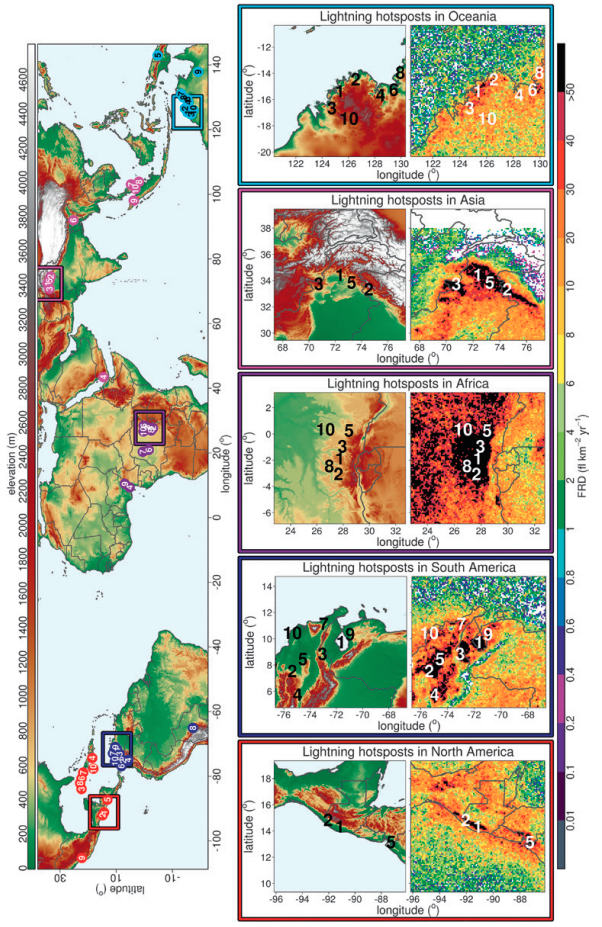
\includegraphics[scale=0.7]{figures/hotspots.png}
  %  \caption{Caption}
   % \label{fig:my_label}
%\end{figure}

%%%%%%%%%%%%%%%%%%%%%%
%%%%% CHAPTER 2  %%%%%
%%%%%%%%%%%%%%%%%%%%%%

\chapter{Fenómenos Luminosos Transitorios en la alta atmósfera}\label{fenomenos}
Las emisiones cortas de luz ocurriendo por encima de las tormentas eléctricas, se empezaron a reportar hace más de 130 años, cuando MacKenzie y Toynbee describieron en 1886 \cite{FullekrugEtal2006} lo que hoy sería conocido como un \textit{Jet Gigante}. Años más tarde se capturaron las primeras imágenes de un \textit{Sprite}, cuando Winckler y sus estudiantes estaban probando un \textit{Low-Light Television} (LLTV) para un próximo vuelo con cohetes de investigación en 1990 \cite{FranzEtal1990}, por lo que se instauró un programa de mapeo de rayos con cámaras similares a los LLTV en el Transbordador Espacial. En este caso los vídeos revelaron un brillo transitorio que se iba ensanchando --seguramente un ELVES-- y más de una docena de rayos ascendentes sobre una tormenta \cite{BoeckEtal1992, Lyons1994A}. A partir de 1993 la NASA comenzó a financiar investigaciones terrestres y aéreas en este campo. En ese período se instaló el mismo LLTV de Winclker en la YRFS (\textit{Yucca Ridge Field Station}), donde se detectaron alrededor de 250 eventos durante varias horas por encima de una tormenta \cite{Lyons1994A, Lyons1994B}. Adem\'as, se descubri\'o que estos eventos produc\'ian señales de audio en la banda VLF \cite{FullekrugEtal2006}. Al año siguiente se produjeron las primeras imágenes a color de los \textit{Sprites} y aparecieron tambi\'en los \textit{Blue Jets} \cite{SentmanEtal1995}. A partir de las observaciones de la YRFS, realizadas entre 1994 y 1995, se hizo evidente la correlación entre los \textit{Sprites} y los rayos tipo +CG \cite{Lyons1996B}. De los 10.000 eventos confirmados sólo algunos \textit{Sprites} fueron relacionados con rayos -CG \cite{BarringtonEtal1999}.

En 1995, la campaña YRFS confirm\'o las predicciones de Taraneko \cite{TaranenkoEtal1993} sobre los ELVES, que los describía como un brillo intenso muy breve ($<1$ms) producido en la base de la ionosfera, asociado con el Pulso Electromagnético (EMP) de un rayo. Los programas ópticos de la YRFS y el \textit{New Mexico Tech’s Langmuir Lab}, revelaron que las primeras observaciones que se pensaban que eran ELVES, en realidad se trataban del Halo que precede a algunos \textit{Sprites} \cite{FullekrugEtal2006}. 

Para un estudio más fino de la estructura espacial y temporal de los \textit{Sprites}, ELVES y Halos, se utilizan una variedad de sensores fotométricos, como el ``ojo de mosca", cámaras de alta velocidad, cámaras de alta resolución e imágenes telescópicas de alta velocidad \cite{FullekrugEtal2006}. A partir de estas observaciones se estimaron las características de los TLE, como la altitud a la que se producen, su tiempo de vida, tamaño, forma, brillo y la tasa de producción en una tormenta típica. En las secciones siguientes se describen las características más conocidas hasta ahora sobre estos fenómenos. 

\section{\textit{Sprites}} 
Los \textit{Sprites} son grandes ráfagas de luz tenue producidas encima de las tormentas eléctricas, que consisten en una cascada de plasma electrificado de color rojizo en su región superior, con ramificaciones azuladas en su parte inferior. El origen de sus filamentos eléctricos generalmente se produce alrededor de los 70 km a 75 km de altitud \cite{FullekrugEtal2006}. Estas ramas altamente estructuradas, suelen propagarse primero hacia abajo, seguidas de una expansión hacia arriba de luminosidad, con un resplandor más difuso en la parte superior. Generalmente, los filamentos no se extienden más allá de los 40 km \cite{FullekrugEtal2006}. 

Todos los \textit{Sprites} son visualmente diferentes, pero se pueden clasificar según su forma en: los tipo columna (c-\textit{Sprites}) y los tipo zanahoria (z-\textit{Sprites}). Los c-\textit{Sprites} suelen ser muy estrechos, con un ancho del orden de 1 km. Son casi continuos, con filamentos que se extienden hacia abajo y hacia arriba. Estos pueden aparecer en grupos de una docena o más \textit{Sprites}, repartidos en varias decenas de kilómetros. El clásico \textit{Sprite} de ``zanahoria" tiene grupos de filamentos que se estrechan hacia abajo con elementos que se ensanchan hacia afuera en la parte superior \cite{FullekrugEtal2006}. Todavía se desconocen los mecanismos que producen estas formas, así como los detalles de su evolución. En la figura \ref{fig:sprite_evolution} se muestra la evolución temporal de un z-\textit{Sprite} típico.

\begin{figure}[h!]
    \centering
    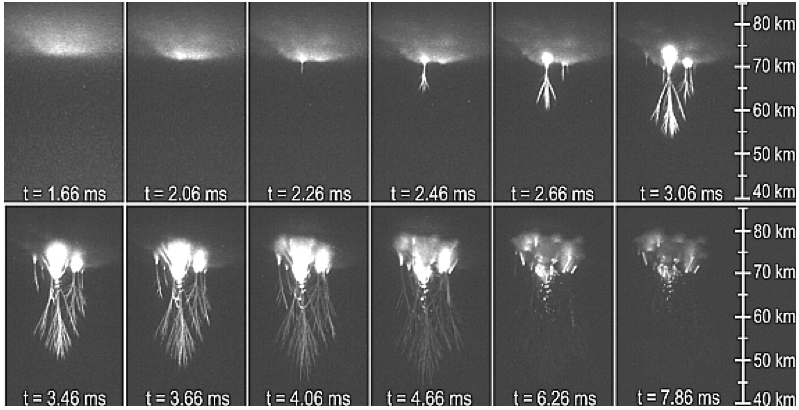
\includegraphics[scale=0.8]{figures/sprite_evolution2.png}
    \caption[Evolución temporal de un Sprite]{Imágenes del desarrollo de la estructura de un z-\textit{Sprite} típico. Las etiquetas de tiempo se refieren al inicio del impacto de retorno del rayo \cite{CummerEtal2006}.}
    \label{fig:sprite_evolution}
\end{figure}

Los \textit{Sprites} ocurren sólo después de las descargas de relámpagos CG con un líder positivo. Estos fenómenos pueden durar desde algunos milisegundos hasta decenas de milisegundos, tiempo suficiente para ser capturados por cámaras, o incluso por el ojo humano \cite{Maiorana2014}. Se estima que el brillo inherente de los \textit{Sprites} está alrededor de 1 MR\footnote{El Rayleigh (R) es una unidad fotométrica para medir emisiones de luz tenue en el cielo que equivale a 10$^{6}$ fotones cm$^{-2}$ columna$^{-1}$ s$^{-1}$ \cite{Hunten1956}.}, con algunos casos raros donde han alcanzado desde 10 MR hasta 30 MR \cite{FullekrugEtal2006}. 

Las diferentes medidas realizadas en la superficie sugieren que se tiene un \textit{Sprite} cada minuto en una tormenta típica. Sin embargo, al occidente de Estados Unidos se han producido desde 400 a 750 \textit{Sprites} en tormentas de 4 a 5 horas \cite{FullekrugEtal2006}.

\section{\textit{Blue Starters}, \textit{Blue Jets}  y \textit{Jets} Gigantes}
Los \textit{Blue Starters} y \textit{Blue Jets}  son rayos que salen del tope de las nubes hacia arriba extendiéndose hasta unos 30 km a 40 km de altitud y luego se desvanecen. Estos eventos tienen forma de cinta, son de color azul y suelen ser más brillantes que los \textit{Sprites} ($>1$ MR). Adem\'as, se propagan con velocidades alrededor de $10^5$ m/s y su tiempo de vida ronda en los 300 ms \cite{DwyerUman2014}. 

Algunos \textit{Jets} se denominan gigantes debido a que pueden alcanzar hasta 70 km de altitud. La forma de un \textit{Jet} Gigante es más compleja, como se observa en la figura \ref{fig:tle_and_tgf}, por lo que generalmente se describen como la mezcla de un \textit{Blue Jet} y un Sprite, debido a que su parte baja es cónica como un \textit{Jet} y luego se dispersa en un brillo difuso y tenue de un tono rojizo como un Sprite. 

Los \textit{Blue Jets} ocurren más o menos con la misma frecuencia que los \textit{Sprites}, mientras que los \textit{Jets} Gigantes son bastante raros, con una tasa de 13 en tres años \cite{chen2008}. Recientemente, se capturaron \textit{Jets} Gigantes con cámaras de alta velocidad en la costa norte colombiana \cite{VanEtal2019}, donde se puede observar claramente el nacimiento y las etapas de evolución de estos fenómenos. En la figura \ref{fig:gigantic_jets_colombia} se aprecia la evolución temporal de un \textit{Jet} Gigante con sus cuatro etapas: el \textit{Jet} líder, el \textit{Jet} completamente desarrollado, el \textit{Jet} de seguimiento y el líder final. 

\begin{figure}
    \centering
    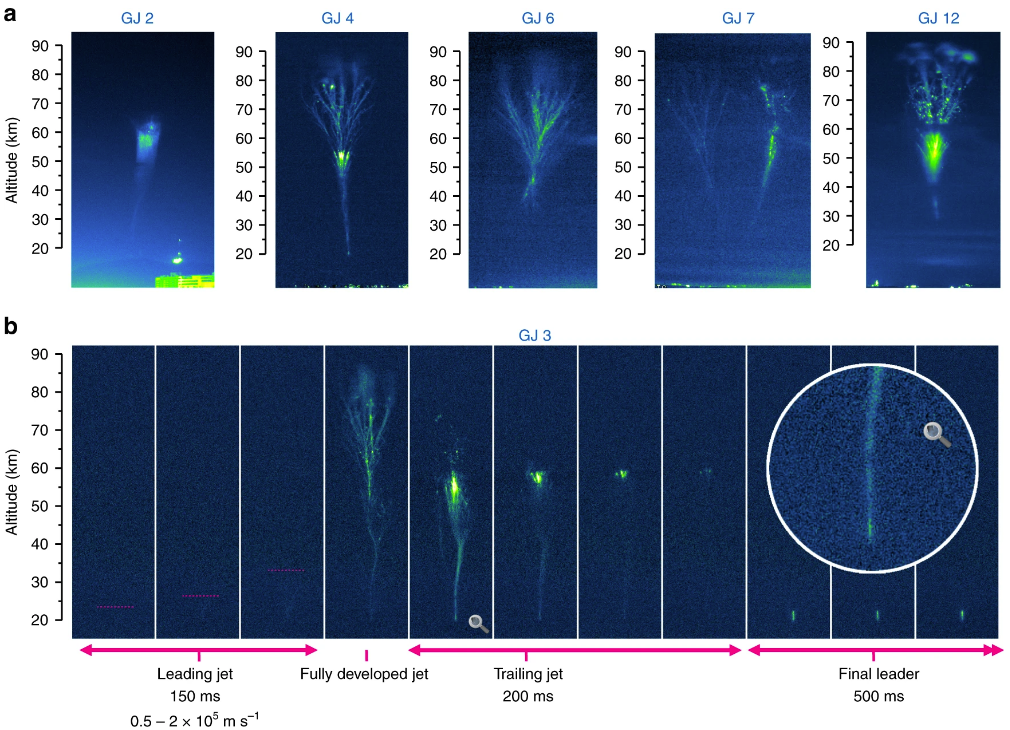
\includegraphics[scale=0.45]{figures/gigantic_jets_colombia.png}
    \caption[\textit{Jets} Gigantes capturados en la costa norte de Colombia]{a) Cinco \textit{Jets} Gigantes capturados en la costa norte de Colombia: Santa Marta (GJ 2-6), Barranquilla (GJ 7) y Cartagena (GJ 12). b) Etapas de la evolución de un \textit{Jet} Gigante grabadas con una cámara de 2.3 mega-píxeles a 20 imágenes por segundo; se puede observar el \textit{Jet} líder en los primeros 150 ms seguido del \textit{Jet} completamente desarrollado, el \textit{Jet} de seguimiento y el líder final \cite{VanEtal2019}.}
    \label{fig:gigantic_jets_colombia}
\end{figure}

\section{ELVES}
Un ELVES es un disco toroidal de luz roja de rápida expansión, que se genera en la parte baja de la ionosfera (la altitud está entre los 80-100 km). Típicamente son generados por el pulso electromagnético de una descarga -CG y su diámetro puede extenderse hasta más de 300 km. El EMP se propaga como una onda esférica desde la base del canal del rayo, intersectando la ionosfera inferior como un anillo que se expande más rápido que la velocidad de la luz en ese medio. El campo eléctrico del EMP produce la calefacción de electrones libres, aumentando las excitaciones inducidas por colisión, la ionización y las emisiones de luz óptica \cite{FullekrugEtal2006}.

El nombre ELVES era originalmente un acrónimo de \textit{Emission of Light and Very low frequency perturbations due to Electromagnetic pulse Sources}, aunque ahora pocos autores mencionan este nombre completo. Estos fenómenos pueden ser tan brillantes como un \textit{Sprite} típico ($\sim$1MR) pero su duración ($\sim$1 ms) hace que sean imperceptibles para el ojo humano y difíciles de capturar con cámaras de vídeo. Es por esto que generalmente se detectan a partir de arreglos de fotómetros, con resoluciones temporales del orden de $\mu$s \cite{MussaCiaccio2012} (ver sección \ref{deteccion}). En la figura \ref{fig:elves_photo} se muestra una foto impresionante de un ELVES, acompañado por tres \textit{Sprites} capturados unas horas despu\'es sobre la misma tormenta (tomada por el astrónomo Timo Kantola \cite{makela2010}). 

\begin{figure}
    \centering
    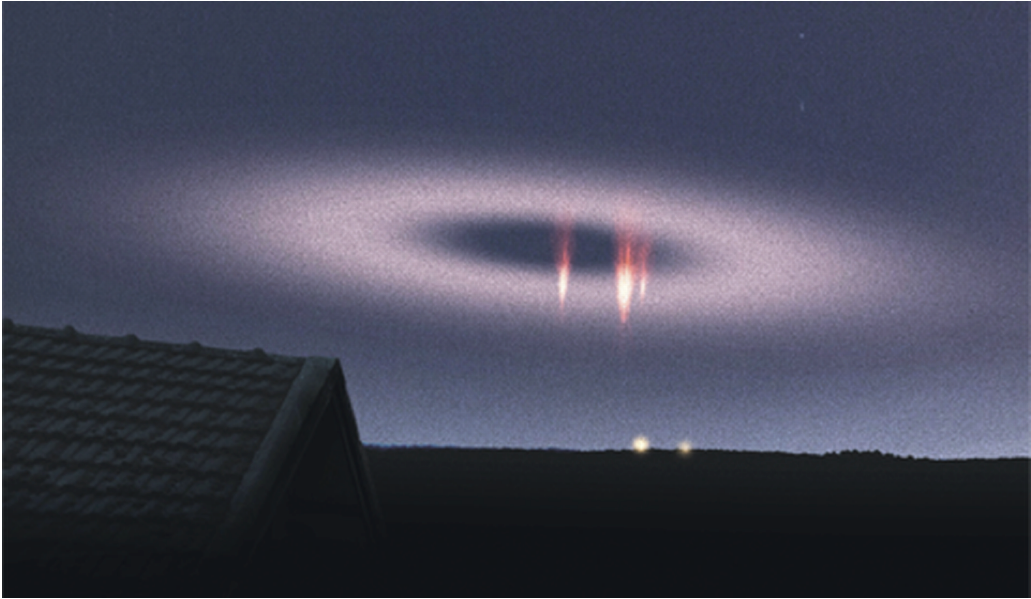
\includegraphics[scale=0.65]{figures/elves_photo.png}
    \caption[Foto de un ELVES tomada por el astrónomo Timo Kantola]{Foto de un ELVES y tres \textit{Sprites} sobre la misma tormenta, tomada por el astrónomo Timo Kantola en Pieksämäki Finlandia \cite{makela2010}.}
    \label{fig:elves_photo}
\end{figure} 

Los ELVES están asociados a descargas -CG con corrientes de pico más altas que la de los rayos que producen los \textit{Sprites}, es decir, mayor a 80 kA. A partir de los datos tomados en tierra, se tiene que los \textit{Sprites} y los ELVES ocurren entremezclados en las mismas tormentas, aunque la proporción varía considerablemente de una tormenta a otra \cite{FullekrugEtal2006}. Por otra parte, las observaciones satelitales de la misi\'on espacial ISUAL (\textit{Imager of Sprites and Upper Atmospheric Lightning}), sugieren que los ELVES son los TLE que ocurren con m\'as frecuencia, con una tasa global de 3.23 eventos min$^{-1}$, superando en número a los \textit{Sprites} (0.50 min$^{-1}$), a los Halos (0.39 min$^{-1}$) y a los \textit{Jets} Gigantes (0.01 min$^{-1}$) \cite{chen2008}, como se observa en la figura \ref{fig:TLE_global_rate}. Estos datos también permitieron concluir que los ELVES ocurren con más frecuencia sobre los océanos que sobre la superficie terrestre, y su tasa aumenta cuando la temperatura de la superficie del mar excede los 26$^{\circ}$C. Esto puede ser debido a que los rayos con corrientes de pico altas ($>80$kA) son más comunes sobre los océanos que sobre la tierra \cite{chen2008}. 

\begin{figure}
    \centering
    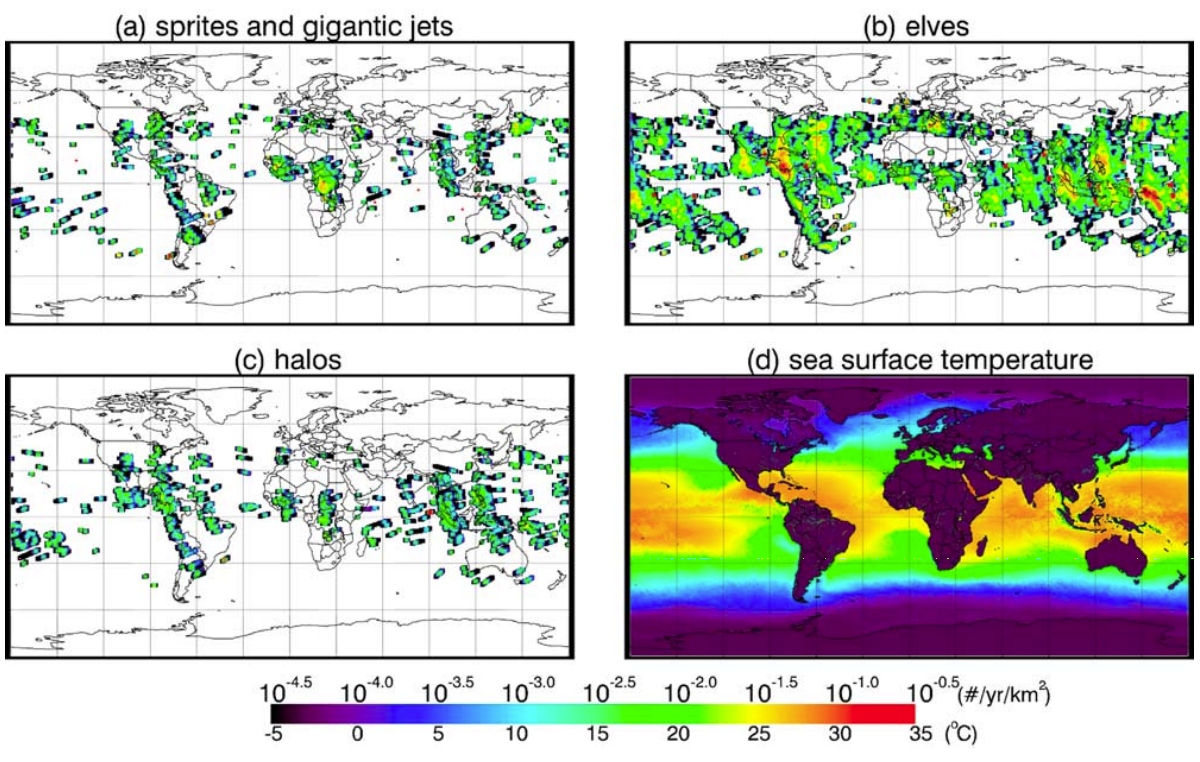
\includegraphics[scale=0.33]{figures/TLE_global_rate.png}
    \caption[Densidad de ocurrencia global de los TLE m\'as comunes]{Densidad de ocurrencia global de los TLE m\'as comunes: (a) \textit{Sprites} y \textit{Jets} Gigantes, (b) ELVES y (c) Halos. Se puede observar que los ELVES son m\'as frecuentes que los \textit{Sprites}, seguidos de los Halos y los \textit{Jets} Gigantes. (d) Se presenta la temperatura de la superficie del mar entre julio de 2004 y diciembre de 2005, para compararla con la densidad de ocurrencia de los ELVES (tomado de \cite{chen2008}).}
    \label{fig:TLE_global_rate}
\end{figure}

\section{Halos}
Son emisiones de luz difusa en forma de disco, que ocurren dentro de un campo eléctrico cuasiestático como los \textit{Sprites}. Al principio estos discos se confundían con ELVES y como aparecían junto a los \textit{Sprites} solían llamarlos \textit{Sprelves}. Ahora se sabe que los Halos pueden aparecer junto con los \textit{Sprites} o por sí solos. De hecho, en una campaña de sensores ópticos en globos \cite{BeringEtal2004}, se observó que muchos Halos asociados a rayos +CG iban acompañados de \textit{Sprites}, a diferencia de los Halos asociados a rayos -CG.

Además, su diámetro es mucho menor que el de los ELVES --máximo de 100 km-- y su duración es mayor (alrededor de 1 ms). Estos eventos se producen por debajo de los ELVES, entre los 65 km y 80 km de altitud. Vídeos de alta velocidad \cite{ArmstrongLyons2000, StanleyEtal1999, StenbaekEtal2000} han demostrado que el Halo es un resplandor amorfo descendente en forma de lente que se inicia típicamente uno o dos milisegundos después del impacto de retorno, y persiste de uno a tres milisegundos. Su brillo es rojo y ronda entre los 0.5 MR y 1 MR \cite{FullekrugEtal2006}.

\section{Destellos de Rayos Gamma Terrestres}
Los Destellos de Rayos Gamma Terrestres son emisiones transitorias breves, que duran menos de unos pocos milisegundos y los fotones emitidos alcanzan energ\'ias de decenas de MeV \cite{neubertEtal2020}. Los TGF son producidos por la radiación de Bremsstrahlung de electrones acelerados en los campos eléctricos de las tormentas, alcanzando energías relativistas en el régimen de escape libre. Los electrones en este régimen pueden ser liberados por las interacciones de los Rayos Cósmicos con la atmósfera, o por los electrones térmicos acelerados en los campos el\'ectricos de los rayos \cite{neubertEtal2020}. Este fenómeno ha sido observado por sat\'elites que pasan sobre las tormentas, como el CGRO (\textit{Compton Gamma-Ray Observatory}) \cite{FishmanEtal1994}, el RHESSI (\textit{Reuven Ramaty High Energy Solar Spectroscopic Imager}) \cite{Smith2005Etal}, m\'as recientemente el sat\'elite AGILE (\textit{Astro-rivelatore Gamma a Immagini Leggero}) \cite{MarisaldiEtal2010}, el Fermi GBM (\textit{Gamma-ray Burst Monitor}) \cite{RobertsEtal2018} y el ASIM (\textit{Atmosphere‐Space Interactions Monitor}) \cite{neubertEtal2019} a bordo de la Estaci\'on Espacial Internacional (ISS).

Inicialmente se pensaba que los TGF se originaban de los TLE de gran altitud, pero más tarde se observó que su fuente estaba dentro de las nubes de tormenta. De hecho, se ha demostrado que \'estos se producen en los primeros pasos del líder inicial de las descargas IC y que algunas emisiones de radio de LF podr\'ian venir directamente del TGF \cite{LyuEtal2018}. Adem\'as, se han identificado emisiones de radio (provenientes de rayos asociados a TGF) que muestran el primer escenario claro de los procesos del rayo que ocurren antes, durante y después de la producción del TGF. En estas observaciones, todos los TGF se produjeron varios milisegundos después de que el líder se iniciara y cuando los líderes alcanzaron de 1 a 2 km de longitud \cite{CummerEtal2015}.

Recientemente, el ASIM observ\'o simultáneamente un TGF y emisiones UV asociadas a un ELVES. El escenario propuesto es el siguiente: el TGF se produce en la etapa inicial del rayo cuyo pulso de corriente genera un ELVES. Las mediciones sugieren que el inicio de la corriente es rápido y de gran amplitud, un prerrequisito para producir los ELVES, y que el TGF se genera en los campos eléctricos asociados al líder del rayo. Esto sugiere que, después de todo, existe una conexión entre los TLE y los TGF \cite{neubertEtal2020}. 


%%%%%%%%%%%%%%%%%%%%%%
%%%%% CHAPTER 3  %%%%%
%%%%%%%%%%%%%%%%%%%%%%
\chapter{Detección global de los ELVES}\label{deteccion}
La primera observación clara de un ELVES se hizo a partir de una cámara de alta velocidad a bordo del Transbordador Espacial en su misión STS-41 (1990) \cite{BoeckEtal1992}. Estos dispositivos son lo suficientemente sensibles para detectar las emisiones de luz en el aire, puesto que una simple molécula de nitrógeno ionizada emite luz a 427nm y 391nm, y la cámara es sensible a longitudes de onda entre los 360 y 720 nm, con un pico de sensibilidad en 440 nm. En este caso, el vídeo fue grabado en formato blanco y negro, con una resolución temporal de $\approx 17$ ms. La imagen fue mejorada restando el fondo y expandiendo la escala de grises, para determinar si el aumento en el brillo era una fluctuación aleatoria o la luminosidad de un rayo. Este ELVES fue observado a una altitud alrededor de los 95 km, en coincidencia con un rayo producido en una tormenta oceánica directamente debajo \'este  \cite{BoeckEtal1992}.  

Más adelante, estos fenómenos se empezaron a estudiar a partir de arreglos lineales de fotómetros, con un tiempo de resolución mejorado a $40\,\mu$s. El campo de visión individual de cada uno de los fotómetros dispuestos en un arreglo horizontal \cite{InanEtal1997}, originaron las primeras medidas de la expansión lateral rápida de la luminosidad óptica de los ELVES, con una resolución temporal de $30\,\mu$s . 

Por otra parte, el experimento ISUAL \cite{chen2008} --a bordo del sat\'elite FORMOSAT-2-- se diseñó para detectar diferentes TLE a través de foto-multiplicadores (PMT) convencionales y multi-ánodos, con resoluciones temporales de 100 y $50\,\mu$s respectivamente. Los datos registrados por ISUAL desde julio de 2004 a junio de 2007 (5.434 ELVES, 633 \textit{Sprites}, 657 Halos y 13 \textit{Jets} Gigantes) permitieron concluir que los ELVES ocurren con m\'as frecuencia respecto a los demás TLE, como se observa en la figura \ref{fig:TLE_global_rate}. Otras misiones espaciales que incluyen observaciones de ELVES en sus programas son TARANIS (\textit{Tool for the Analysis of Radiation from lightning and Sprites}) \cite{lefeuvre2008taranis} y \textit{Firefly} \cite{rowland2011nsf}. \textit{TARANIS} se enfoca en estudiar las regiones donde se originan los TLE y TGF, sus mecanismos de generación, los fenómenos asociados, así como el estudio de los parámetros de entrada para modelar la variación de la atmósfera y el CGE. Por su parte, \textit{Firefly} emplea nano-satélites diseñados para explorar la relación entre los rayos y los TGF, para descifrar qué tipos de rayos producen estos haces de electrones y los TGF asociados.

El ASIM, \cite{neubertEtal2019} a bordo de la Estaci\'on Espacial Internacional, comprende la primera misión espacial con un conjunto completo de instrumentos diseñados para medir rayos, TLE y TGF. ASIM se desarroll\'o en el marco de la Agencia Espacial Europea y fu\'e lanzado en abril de 2018, contando con un monitor de rayos X y rayos gamma que mide fotones de 15 keV a 20 MeV, y un conjunto de tres fotómetros y dos cámaras que miden en las bandas de 180-250 nm, 337 nm y 777.4 nm. Sus objetivos fundamentales son el conteo mundial exhaustivo de TLE y TGF abarcando todas las horas nocturnas y estaciones locales; toma de datos para comprender los procesos cinéticos fundamentales de los TLE y TGF; y entender la relación de los TLE y los TGF con la actividad de los rayos.

%Otros objetivos adicionales que pueden abordarse con los instrumentos se relacionan con la física espacial, como las auroras y los meteoros, y con la observación de la Tierra, como los efectos del polvo y el aerosol en la electrificación de las nubes. 

Mientras que estas misiones fueron desarrolladas específicamente para el estudio de rayos, TGF y TLE, el Detector de Fluorescencia del Observatorio Pierre Auger descubrió por accidente un candidato a ELVES durante un turno de observación en el año 2005 \cite{Mussa2019}. Este observatorio, ubicado en Malargue, Argentina, es el más grande del mundo en infraestructura para el estudio de Rayos Cósmicos de ultra-alta energía, que combina las facilidades de un Detector de Superficie (SD) y un Detector de Fluorescencia (FD). Además de su actividad principal, el observatorio inició un programa de estudios en Cosmo-geofísica, para explotar las características de su FD en el estudio de eventos luminosos transitorios. El FD permite la detecci\'on de ELVES en un \'area de $3 \times 10^{6}$ km$^2$ \cite{aab2020}, abarcando zonas sobre los océanos Pacífico y Atlántico, así como la región de Córdoba en Argentina, conocida por sus fuertes tormentas de convección. El Observatorio Pierre Auger podría ser el mejor instrumento con bases en la tierra para la observación de eventos en la banda del ultravioleta cercano \cite{MussaCiaccio2012}, por lo que a continuación se describe su funcionamiento.  

%%%%%%%%%%%%%%%%%%%%%%%%%%%%%%%%%%%
%%%%%%%%%%%%%%%%%%%%%%%%%%%%%%%%%%%
\section{ELVES en el Observatorio Pierre Auger}
\begin{figure}
    \centering
    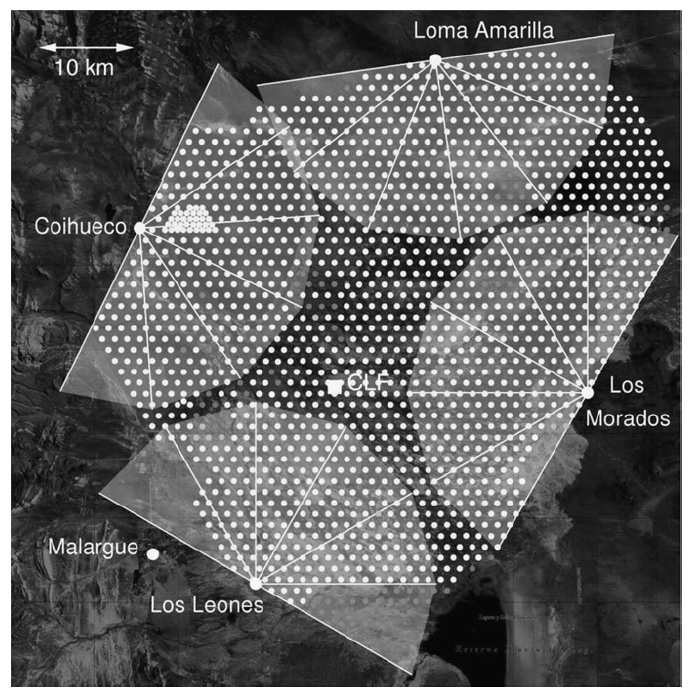
\includegraphics[scale=0.5]{figures/auger_sites.png}
    \caption[Distribuci\'on de los Detectores de Superficie y Fluorescencia del Observatorio Pierre Auger.]{Distribuci\'on de los Detectores de Superficie y de Fluorescencia del Observatorio Pierre Auger. Los puntos grises muestran las posiciones de las estaciones del SD, mientras que las l\'ineas indican el campo de visi\'on de los 24 telescopios del FD. Los telescopios est\'an ubicados en el per\'imetro del SD en cuatro edificios: Los Leones, Los Morados, Loma Amarilla y Coihueco \cite{AbrahamEtal2010}. }
    \label{fig:auger_sites}
\end{figure}
El detector de Fluorescencia del Observatorio Pierre Auger consta de cuatro sitios de observaci\'on localizados en la cima de pequeñas colinas (Los Leones, Los Morados, Loma Amarilla y Coihueco), en los límites del arreglo del SD (ver figura \ref{fig:auger_sites}). Los cuatro edificios del FD contienen seis telescopios independientes, cada uno con un campo de visión de 30 grados en acimut $\times$ 30 grados de elevación (ver figura superior de \ref{fig:fd_scheme}). La combinación de los seis telescopios cubre 180 grados en acimut \cite{AbrahamEtal2010}. En cada telescopio, la luz entra a través de una ventana con un filtro UV y es enfocada a través de un espejo esférico segmentado sobre la cámara. Los elementos del telescopio se muestran en la parte inferior izquierda de la figura \ref{fig:fd_scheme}. Las c\'amaras de los telescopios est\'an compuestas de 440 PMT hexagonales en un arreglo matricial de 22 filas por 20 columnas como se muestra en la figura c de \ref{fig:fd_scheme}. Estos PMT representan los p\'ixeles de la c\'amara y est\'an ubicados sobre una superficie esf\'erica con pasos de 1.5$^\circ$ \cite{AbrahamEtal2010} (ver figura a y b de \ref{fig:fd_scheme}). 

La longitud de onda de la luz detectada en cada PMT var\'ia desde 300 nm hasta 420 nm y los pulsos de luz se digitalizan cada 100 ns. Para la selección en línea de los eventos, la data de cada PMT es procesada a través de un sistema de disparo de tres etapas \cite{MussaCiaccio2012}. Los 24 telescopios del FD son ideales para la observación de los ELVES, pero para la selecci\'on en línea de estos eventos con una eficiencia razonable, se han realizado estudios basados en sub-triggers auxiliares que permitieron modificar el tercer nivel del sistema de disparo \cite{Mussa2019}.

\begin{figure}
    \centering
    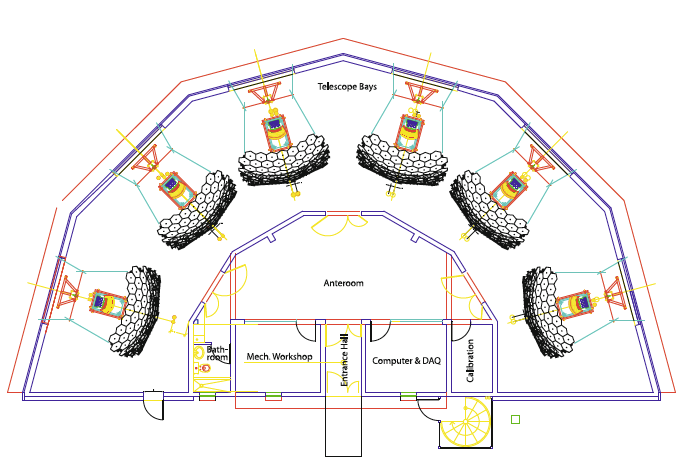
\includegraphics[scale=0.5]{figures/eye_scheme.png}
    
    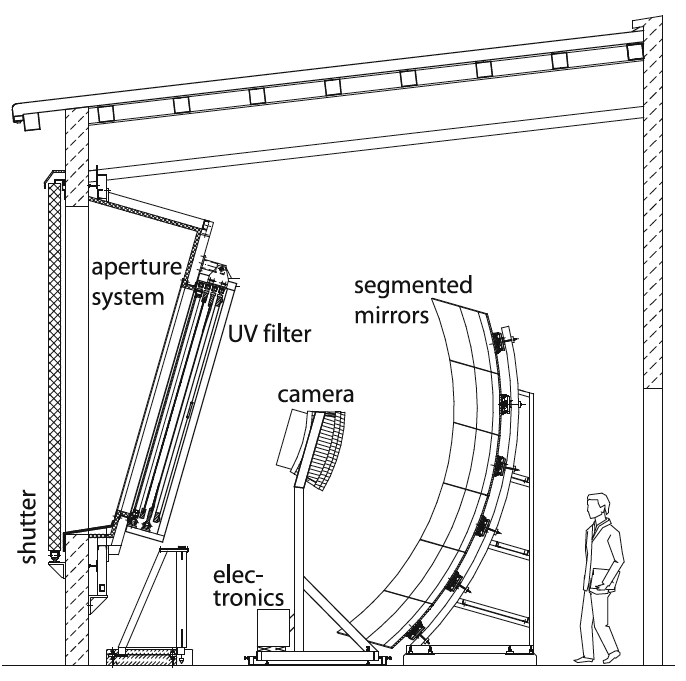
\includegraphics[scale=0.35]{figures/telescope_scheme.png} \,\,\, 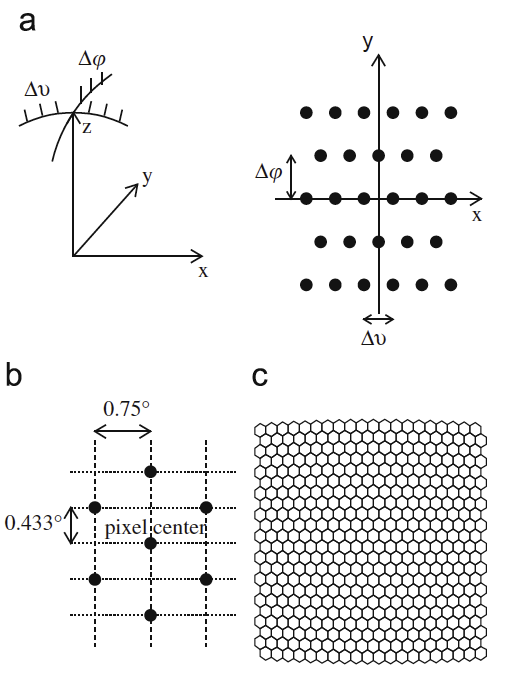
\includegraphics[scale=0.35]{figures/camera.png}
    \caption[]{Arriba: estructura de los edificios del FD con seis telescopios de fluorescencia independientes. Cada uno tiene un campo de visión de 30 $\times$ 30 grados en acimut y elevación, que en total cubren 180 grados en acimut. Abajo, a la izquierda: estructura y componentes de los telescopios de cada FD; a la derecha: construcci\'on geom\'etrica de las c\'amaras del FD: a) los centros de los píxeles est\'an ubicados sobre una superficie esf\'erica en pasos de 1.5 grados, b) posicionamiento de los vértices del píxel respecto a su centro, y c) arreglo de los 440 píxeles de la c\'amara en una matriz de 22 $\times$ 20. Tomado de \cite{AbrahamEtal2010}.}
    \label{fig:fd_scheme}
\end{figure}

%%%%%%%%%%%%%%%%%%%%%%%%%%%%%%%%%%%
\subsection{Sistema de disparo del FD}
El disparador del FD está estructurado en tres niveles \cite{Mussa2019}: 
\begin{enumerate}
    \item El disparo del primer nivel (DPN) opera a nivel del píxel, con un umbral ajustable que mantiene la tasa de activación de los PMT a 100 Hz.
    \item El disparo del segundo nivel (DSN) busca segmentos con trayectorias de al menos 5 píxeles adyacentes que pasaron la primera etapa. 
    \item El disparo del tercer nivel (DTN) está diseñado para excluir eficientemente los rayos cercanos. Los eventos de rayos presentan una alta multiplicidad de píxeles disparados que se distribuyen de forma aleatoriamente temporal a través de la cámara, dentro de una ventana de tiempo de 100 $\mu$s. 
\end{enumerate}

El DTN basado en la multiplicidad, instalado a finales del 2007 como reemplazo de una versi\'on previa menos eficiente, permiti\'o el hallazgo inesperado de ELVES en los primeros datos del Observatorio Pierre Auger \cite{MussaCiaccio2012}). Después de un estudio de cuatro años de eventos de DPN, el DTN se modificó y arrojó 58 nuevos candidatos de ELVES \cite{Mussa2019}.

El nuevo DTN verifica la evoluci\'on angular del frente de luz alrededor del primer p\'ixel disparado. Para un conjunto de p\'ixeles de la misma columna que \'este, el algoritmo requiere que al menos dos p\'ixeles antes y dos p\'ixeles desp\'ues del central tengan un pulso. Adem\'as, 80\% de \'estos deben mostrar un incremento en el tiempo del pulso. En comparación con los Rayos Cósmicos, los ELVES depositan una gran cantidad de luz, por lo que es necesario al menos un píxel con un pulso de amplitud mayor que 50 cuentas ADC \cite{Mussa2019}. En la figura \ref{fig:crs_elves} se puede observar un Rayo C\'osmico registrado en la c\'amara como una l\'inea de p\'ixeles activados con un patr\'on geom\'etrico y una clara secuencia temporal, mientras que el ELVES se ve como un frente de onda con una evolución radial. 

\begin{figure} 

    \centering
    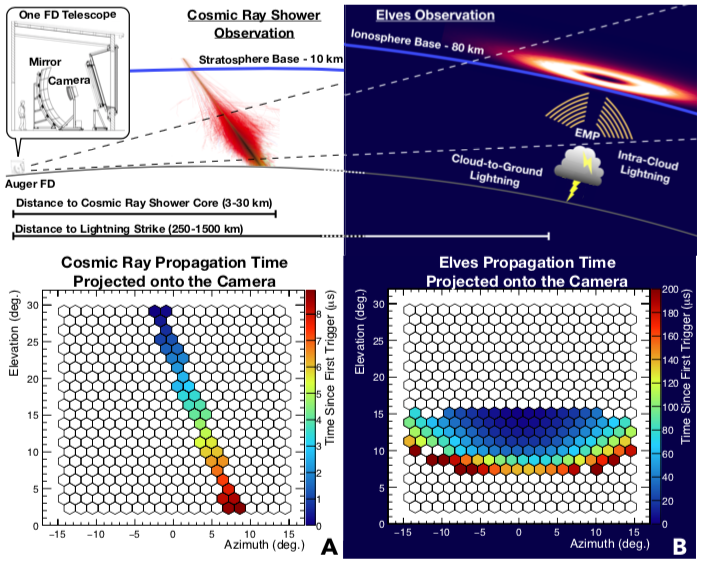
\includegraphics[scale=0.6]{figures/cr_vs_elves.png}
    \caption[Observaci\'on de Rayos C\'osmicos y ELVES en un telescopio del FD del Observatorio Pierre Auger]{Observaci\'on de Rayos C\'osmicos y ELVES en un telescopio del FD. Tiempo de propagaci\'on proyectado sobre la c\'amara
    de A) un Rayo C\'osmico y B) un ELVES. El tiempo se mide a partir del primer disparo del sistema, siendo los p\'ixeles azules los primeros en activarse y los rojos los \'ultimos. Se puede observar que el Rayo C\'osmico activa una l\'inea de p\'ixeles con una clara secuencia temporal y que el ELVES se ve como un frente de onda con una evolución radial.}
    \label{fig:crs_elves}
\end{figure}

Desde el 2013, el Observatorio Pierre Auger ha estado tomando datos con este sistema de disparo para el estudio de ELVES. Durante el primer año se observ\'o que las trazas estándar del FD, de 72 $\mu$s de largo, no permit\'ian ver la luz emitida desde la regi\'on de la ionosfera localizada verticalmente sobre el rayo fuente. Entonces, se modific\'o el esquema de lectura del FD (denominado \textit{Extended Readout}) para adquirir tres cuadros consecutivos en estos casos especiales. Este cambio permite el estudio de la distribuci\'on angular de la emisi\'on de luz por encima del rayo. Los datos de ELVES desde 2014 hasta 2016 se tomaron con una traza m\'axima de 300 $\mu$s de longitud. A partir del 2017, esta traza se extendi\'o hasta 900 $\mu$s para observar completamente la regi\'on de alta intensidad de luz en la mayor\'ia de los eventos \cite{Mussa2019}. Hasta septiembre del año 2018 se han registrado m\'as de 4000 ELVES en el Observatorio Pierre Auger, como se muestra en el cuadro \ref{eventos_elves}, donde los observados en un solo sitio del FD se denominan Simples, en dos sitios son los Estéreo y en tres sitios los Tripletes.  

\begin{table}[]\centering
\caption{N\'umero de ELVES registrados en el FD desde el 2013 hasta el 2018 \cite{Mussa2019}}
\label{eventos_elves}
\begin{tabular}{lcccc}
\rowcolor[HTML]{EFEFEF} 
Año         & Simple & Estéreo & Triplete & Total                        \\
2013 (4-12) & 214    & 83      & 8        & \cellcolor[HTML]{EFEFEF}305  \\
2014        & 425    & 128     & 19       & \cellcolor[HTML]{EFEFEF}572  \\
2015        & 686    & 117     & 11       & \cellcolor[HTML]{EFEFEF}814  \\
2016        & 673    & 151     & 21       & \cellcolor[HTML]{EFEFEF}845  \\
2017        & 906    & 297     & 52       & \cellcolor[HTML]{EFEFEF}1255 \\
2018 (1-9)  & 527    & 99      & 15       & \cellcolor[HTML]{EFEFEF}641  \\
\rowcolor[HTML]{EFEFEF} 
Total       & 3431   & 875     & 126      & 4432                        
\end{tabular}
\end{table}

%%%%%%%%%%%%%%%%%%%%%%%%%%%%%%%%%%%
\subsection{Reconstrucci\'on de la ubicaci\'on y la emisi\'on de luz de los ELVES }
La reconstrucción apunta a la localización precisa en tiempo y espacio del rayo que origin\'o el ELVES, y a la medición de la distribución angular de la emisión de luz desde la base de la ionosfera. Para esto, lo primero que se hace es un ajuste de una o m\'as gaussianas asim\'etricas a la traza ADC de cada uno de los píxeles. La reconstrucci'on de la ubicaci'on del rayo es un proceso de cuatro pasos \cite{Mussa2019}:
\begin{enumerate}
    \item Se realiza un conjunto de ajustes polinomiales en los tiempos $T_i$ del pulso de cada fila y cada columna, para obtener una primera estimaci\'on de la longitud y la latitud del rayo. 
    
    \item Se realiza otro ajuste para minimizar el $\chi ^{2}= \sum_{i=1}^{N} \left( T_i -\Delta T_0 -\overline{OPS}_i/c \right)^{2}$, donde $\Delta T_0$ es el tiempo entre la emisión del EMP de la fuente y la observación de la primera luz en el diafragma del FD, $\overline{OPS}_i$ es la suma de las distancias $\overline{\text{SP}}$ y $\overline{\text{PO}}$ (ver figura \ref{fig:emission_layer}). En este caso se asume que la capa de emisión no tiene grosor y que la altitud es $H_{EM}=92$ km.
    
    \item El tercer ajuste se hace dejando libre la altitud de emisión $H_{EM}$.
    
    \item El último ajuste se realiza permitiendo también que la altitud del rayo $H_B$, varíe sobre el nivel del mar.
\end{enumerate}
\begin{figure}
    \centering
    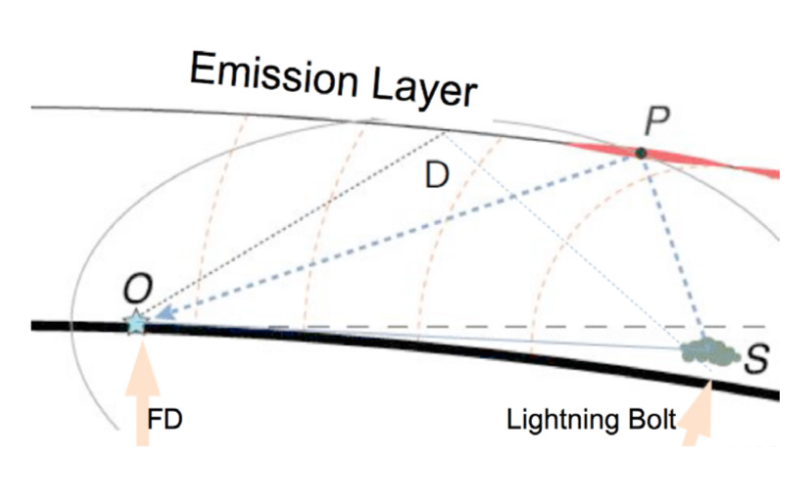
\includegraphics[scale=0.3]{figures/emission_layer.png}
    \caption[Geometr\'ia de reconstrucci\'on de los ELVES en el Observatorio Pierre Auger]{Geometr\'ia de reconstrucci\'on de los ELVES en el Observatorio Pierre Auger \cite{Mussa2019}. $\overline{\text{SP}}$ es la distancia de la fuente del EMP (S) a la capa de emisi\'on donde se produce el ELVES y $\overline{\text{PO}}$ es la distancia desde la capa de emisi\'on hasta el FD del observatorio. En el proceso de reconstrucci\'on se asume que la capa de emisi\'on no tiene grosor \cite{Mussa2019}.}
    \label{fig:emission_layer}
\end{figure}

Después de haber localizado el rayo fuente, se procede a calcular la cantidad total de fotones irradiados por el ELVES. Para esto es necesario transformar la cantidad de luz observada en cada píxel, $P_i(FD)$, a la densidad superficial de fotones ,$\Phi_i$, en la base de la ionosfera:
\begin{equation}
    \Phi_i=P_i(FD)\times C_i(geom)\times C_i(atmo).
\end{equation}
La corrección geométrica, $C_i(geom)$, tiene en cuenta el ángulo sólido entre el diafragma del FD y el tamaño de la superficie emisora en la base de la ionosfera ($A_{emis}$):
\begin{equation}
    C_i(geom)=\frac{\overline{OP}^{2}}{A_{mirror}A_{emis}}.
\end{equation}

Por otra parte, la corrección atmosférica incluye las profundidades ópticas, $\tau$, de los aerosoles y las moléculas a través del camino de la luz:
\begin{equation}
    C_i(atmo)= \exp\left(-(\tau_{OP, mol}+\tau_{OP, aer})\times AM(\theta)\right),
\end{equation}

donde $AM(\theta)$ es la masa de aire. 

La corrección geométrica y la atmosférica dependen fuertemente del número de fila y débilmente del número de columna de la cámara. Después de aplicar estas correcciones, en el caso de un dipolo perfecto, la distribución angular de la emisión es azimutalmente simétrica con respecto a la vertical del rayo, y la cantidad total de luz emitida desde la base de la ionosfera puede extrapolarse fácilmente a partir de la fracción observada. Sin embargo, se necesita más trabajo para modelar dipolos inclinados o patrones de emisi\'on m\'as complejos \cite{Mussa2019}.


%%%%%%%%%%%%%%%%%%%%%%%%%%%%%%%%%%%
\subsection{Clasificación de ELVES múltiples}
\begin{figure}
    \centering
    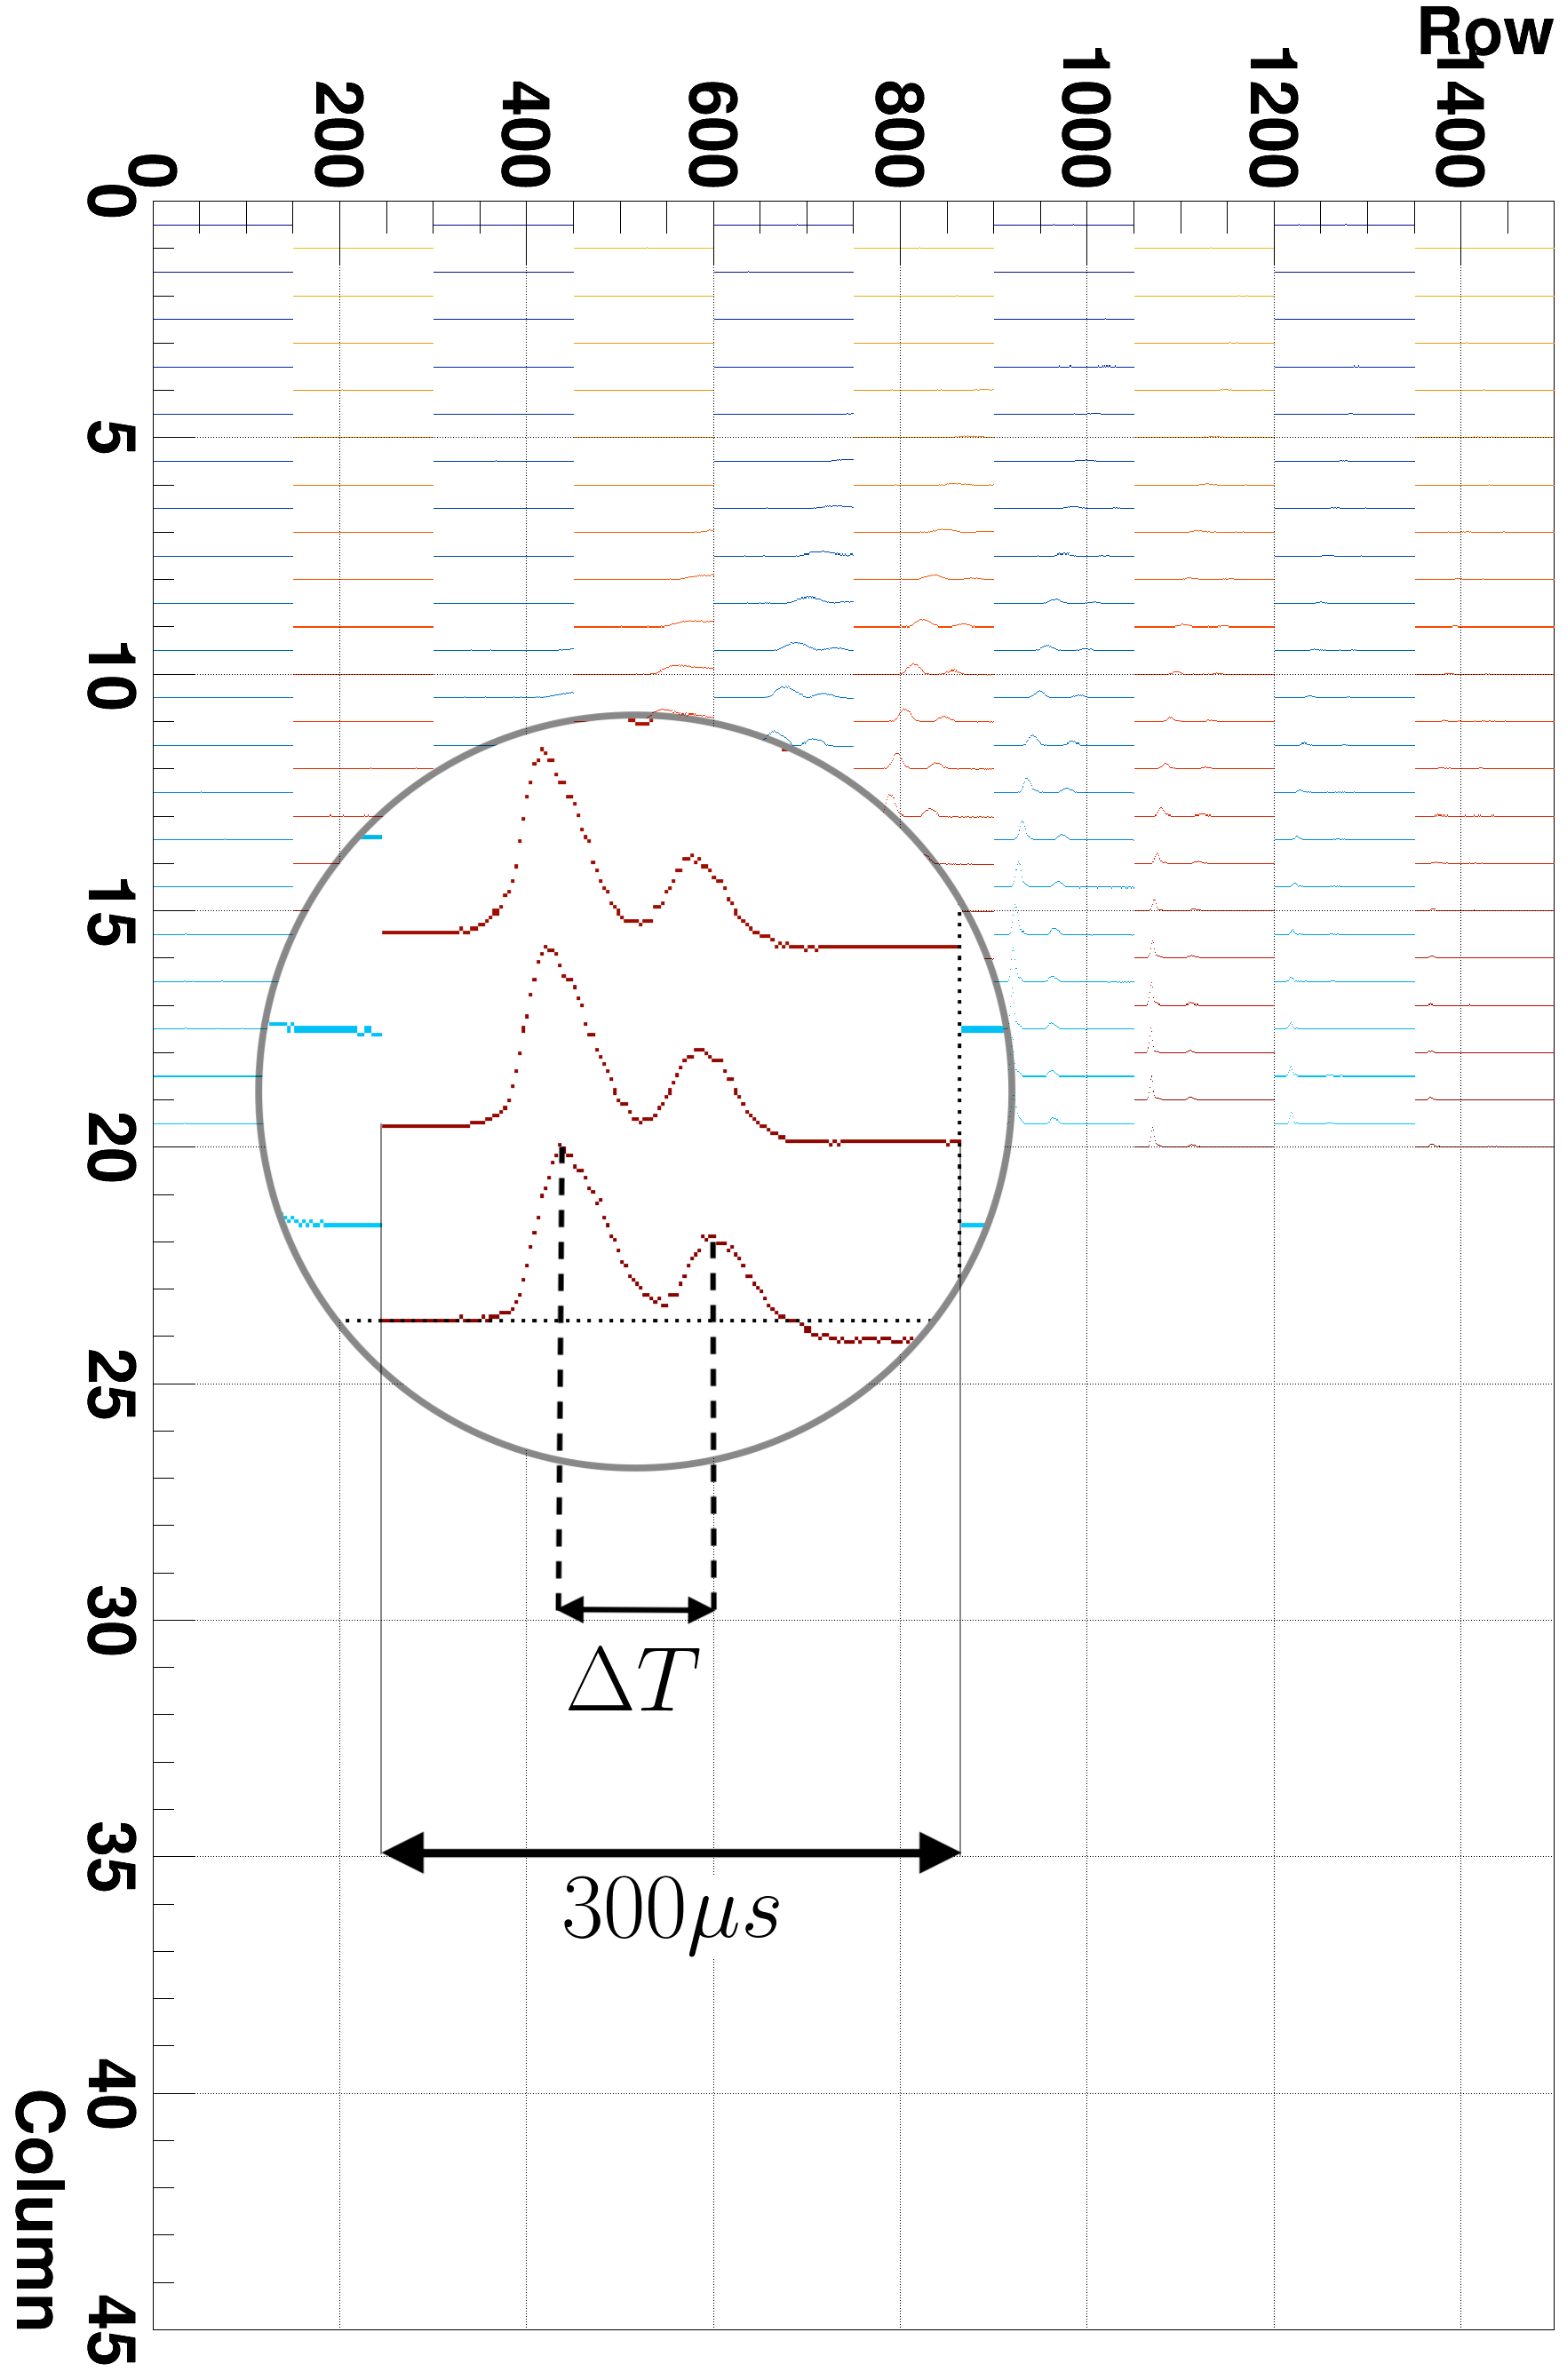
\includegraphics[scale=0.1]{figures/double_elves_1.png}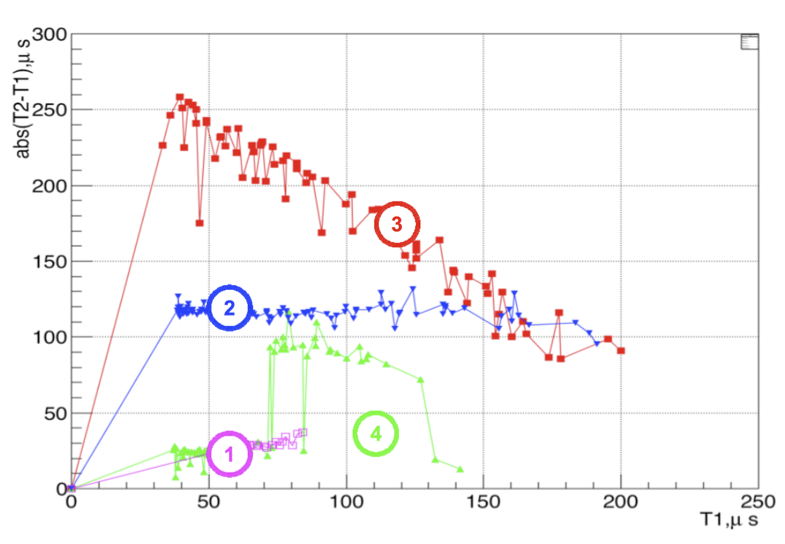
\includegraphics[scale=0.7]{figures/categorias.png}
    \caption[Clasificaci\'on de los ELVES m\'ultiples]{Izquierda: ejemplo de un evento con m\'as de diez p\'ixeles donde sus trazas de 300$\mu$s muestran un doble pulso; en la ampliaci\'on se puede observar la diferencia temporal $\Delta T$ entre los dos pulsos. Derecha: diferencia temporal entre dos pulsos de una traza, $\Delta T$, versus el tiempo del primer pulso, $T_1$, en eventos de ELVES m\'ultiples clasificados en cuatro categor\'ias \cite{Mussa2019}.}
    \label{fig:categorias}
\end{figure}
En un evento, cuando m\'as de diez p\'ixeles muestran m\'as de un pulso en las trazas (ver figura izquierda de \ref{fig:categorias}) el ELVES se denomina m\'ultiple y se realiza un an\'alisis diferente al descrito anteriormente. El primer paso consiste en graficar la diferencia temporal entre los dos pulsos, $\Delta T$, respecto al tiempo del primer pulso, $T_1$, representado en la figura \ref{fig:categorias} donde estos eventos se pueden clasificar en cuatro categor\'ias \cite{Mussa2019}:

\begin{enumerate}
    \item Cuando $\Delta T$ es constante y muy pequeño ($<50 \,\mu$s) el doble pulso se puede explicar debido a un patrón de interferencia producido por un EMP emitido por un rayo IC, que rebota en el suelo. 
    \item En el caso donde $\Delta T \geq 50\mu$s y es constante, los eventos se pueden relacionar con las primeras etapas del rompimiento inicial de los rayos o con los impactos de retornos muy cercanos. 
    \item La tercera categor\'ia, donde $\Delta T$ es linealmente decreciente con el tiempo del pulso, se puede explicar como un ELVES simple superpuesto con alguna otra clase de luz transitoria, con un tiempo de subida mucho más largo.
    \item En la \'ultima categor\'ia se tienen cambios m\'as abruptos de $\Delta T$ pertenecientes a ELVES con m\'as de dos pulsos en las trazas. Este patr\'on podr\'ia estar asociado a la producci\'on de TGF.
    \end{enumerate}

En el 2008, el \textit{Photometric Imager of Precipitated Electron Radiation} (PIPER) detectó el primer ELVES con dos pulsos \cite{Newsome2010}. Posteriormente se confirmó que la amplia separación temporal entre estos pulsos se correlacionaba con las descargas de rayos compactos entre nubes de gran altitud (CID) \cite{Marshall2015,Lyu2015}. En 2017, se preveía que los ELVES con más de dos pulsos en la traza, separados por un tiempo mucho más corto, se correlacionaban con los Pulsos Energéticos dentro de la nube (EIP), que est\'an asociados a la producci\'on de TGFs \cite{Liu2017,neubertEtal2020}]. 

La mejor\'ia de la sensibilidad de los detectores y el modelado de los rayos, sugiere que las mediciones de ELVES de varios pulsos pueden ser utilizadas para entender mejor el proceso de impacto de retorno de los rayos de los EIPs y los CID, para estudiar el vínculo entre los ELVES y los TGF \cite{Marshall2014,Da2015}. Desde 2014 al 2016 el Observatorio Pierre Auger report\'o 1598 ELVES, que se dividieron en 1310 de pulso simple y 288 con m\'ultiples pulsos compatible con descargas IC \cite{aab2020}. Este observatorio planea seguir operando hasta el 2025, lo que supone un aumento en la base de datos para el análisis de ELVES simples y m\'ultiples, aportando a una mejor comprensi\'on de estos fen\'omenos. 

\bibliographystyle{unsrt}
\bibliography{monografia}

\end{document}